\chapter{Programmbeschreibung}
\label{chap:Programmbeschreibung}
\section{Pakete}
Das Programms ist in drei Module unterteilt, welche nach dem MVC-Model entwickelt wurden. Für jedes dieser Module wurde zunächst ein Interface deklariert, damit das Programm leicht wart- und erweiterbar bleibt. Die Namen der Interfaces beginnen mit einem \glqq I\grqq, wie es etwaige Namenskonventionen vorgeben.
\begin{figure}[!h]
	\centering
	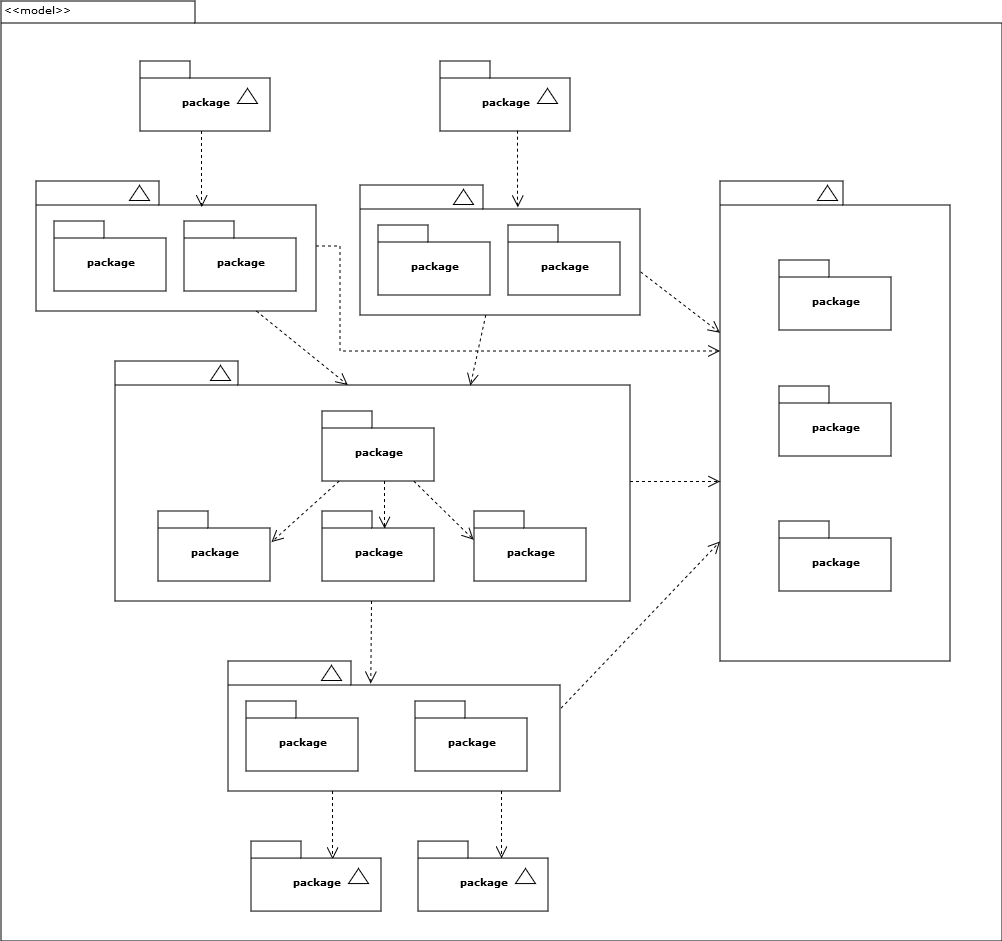
\includegraphics[width=1\textwidth]{./../Diagramme/PackageDiagram.png}
	\caption{Übersicht zu den Paketen}
\end{figure}
\clearpage
\subsection{Model}
%\begin{figure}[!h]
%	\centering
%	\includegraphics[width=0.25\textwidth]{./Graphics/ModelClasses}
%	\caption{Klassendiagramme aus dem Paket Model}
%\end{figure}
\begin{description}
	\item[IModel] Schnittstelle zum Speichern der Daten: Spielsteine, Spielfeld, Matrix der Nachbarschaft für Felder
	\item [Model] Implementierung von \lstinline{IModel}.
\end{description}

\subsection{IO}
\begin{figure}[!h]
	\centering
	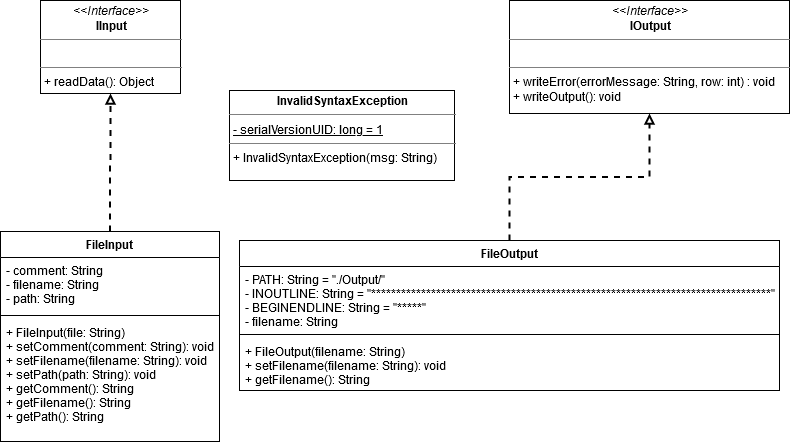
\includegraphics[width=\textwidth]{./../Diagramme/IO-Classdiagram.png}
	\caption{Klassendiagramme aus dem Paket IO}
\end{figure}
\begin{description}
	\item [IInput] Schnittstelle zur Eingabe der Daten.
	\item [FileInput] Implementierung von \lstinline{IInput}. Die Klasse verfügt über eine Methode zum einlesen der Dateien, und eine weitere zur syntaktischen Überprüfung dieser.
	\item [IOutput] Schnittstelle zur Ausgabe der Daten.
	\item [FileOutput] Implementierung von \lstinline{IOutput}. Die Klasse verfügt über zwei Methoden, eine zum schreiben einer einfachen Ausgabedatei, und eine zweite zum schreiben einer Fehlerdatei.
	\item [InvalidSyntaxException] Exception Klasse zum signalisieren, dass ein syntaktischer Fehler in der Eingabedatei vorliegt. Wird in der Klasse \lstinline{FileInput} verwendet.
\end{description}

\subsection{Controller}
%\begin{figure}[!h]
%	\centering
%	\includegraphics[width=0.7\textwidth]{./Graphics/ControllerClasses}
%	\caption{Klassendiagramme aus dem Paket Controller}
%\end{figure}
\begin{description}
	\item [PuzzleLoeserFactory] Schnittstelle zum Starten des Controllers, damit die Verarbeitung gesteuert werden kann.	\item [PuzzleLoeser] Abstrakte Klasse als Schnittstelle zum Starten. \lstinline{PuzzleLoeserEinsetzen}. Beinhaltet die Implementierungen und den Lösungsalgorithmus.
\end{description}

\section{Schnittstellen}
\subsection{Program}
\subsubsection{\underline{Main}}
\lstinline{public static void main(string[] args)}
\begin{description}
	\item [Eingabeparameter:] Array mit den Kommandozeilen-Argumenten
	\item [Rückgabeparameter:] keine
\end{description}

\subsection{Spielstein}
\subsubsection{\underline{drehen}}
\lstinline{public Spielstein drehen();}
\begin{description}
	\item [Eingabeparameter:] keine vorhanden
	\item [Rückgabeparameter:] der gedrehte Spielstein wird zurückgegeben.
\end{description}

\subsubsection{\underline{getFeld}}
\lstinline{public int getFeld();}
\begin{description}
	\item [Eingabeparameter:] keine vorhanden
	\item [Rückgabeparameter:] das Feld, auf dem der Spielstein liegt, ist der Spielstein nicht gelegt, wird 0 zurückgegeben.
\end{description}

\subsubsection{\underline{setFeld}}
\lstinline{public void setFeld(int feld);}
\begin{description}
	\item [Eingabeparameter:] Die Feldnummer, des Feldes, in die der Stein gesetzt wurde.
	\item [Rückgabeparameter:] keiner
\end{description}

\subsubsection{\underline{kannKombi}}
\lstinline{public boolean kannKombi(List<Integer> kombination);}
\begin{description}
    \item [Eingabeparameter:] Eine Liste mit den Kantenziffern, der Nachbarfelder, beginnend mit der Grundkante.
    \item [Rückgabeparameter:] Wenn der Spielstein in der aktuellen Orientierung die Kombination abdecken kann, dann wird \lstinline{true} zurückgegeben, sonst \lstinline{false}.
\end{description}

\subsection{Spielfeld}
\subsubsection{\underline{GetInstance}}
\lstinline{public Spielfeld getInstance()}
\begin{description}
	\item [Eingabeparameter:] keiner
	\item [Rückgabeparameter:] eine Spielfeldinstanz.
\end{description}

\subsubsection{\underline{GetKombination}}
\lstinline{public List<Integer> GetKombination(int feld)}
\begin{description}
	\item [Eingabeparameter:] Die Feldnummer, für das Feld, deren Kombination gesucht ist.
	\item [Rückgabeparameter:] Eine Liste mit Integer-Werten für die Kantenziffer, die an Position x vorhanden sein muss, beginnend von der Grundkante. Liegt an einer Kante noch kein weiterer Stein, wird anstelle der Kantenziffer ein null in der Liste zurückgegeben.
\end{description}

\subsection{DateiBehandlung}
\subsubsection{\underline{SchreibeDatei}}
\lstinline{public void schreibeDatei(List<Spielstein> loesung)}
\begin{description}
	\item [Eingabeparameter:] Eine Liste der Spielsteine, aufsteigend nach den Feldern, in die diese gelegt werden sortiert. Ist keine Lösung vorhanden, wird eine leere Liste übergeben.
	\item [Rückgabeparameter:] keiner
\end{description}

\subsubsection{\underline{SchreibeFehler}}
\lstinline{public void schreibeFehler(String text)}
\begin{description}
	\item [Eingabeparameter:] Die Fehlermeldung die Ausgegeben werden soll, mit vorangestellter Zeile und Datei in der der Fehler festgestellt wurde, getrennt durch \#
	\item [Rückgabeparameter:] keiner
\end{description}

\subsubsection{\underline{LeseDatei}}
\lstinline{public List<Spielstein> leseDatei()}
\begin{description}
    \item [Eingabeparameter:] keine vorhanden
    \item [Rückgabeparameter:] Eine Liste der in der Eingabedatei beschriebenen Spielsteine, sortiert nach der Einlesereihenfolge. Kommt es beim einlesen zu Fehlern, so wird null zurückgegeben.
\end{description}

\subsection{PuzzleLoeser}
\subsubsection{\underline{loesePuzzle}}
\lstinline{public void loesePuzzle()}
\begin{description}
	\item [Eingabeparameter:] keine vorhanden
	\item [Rückgabeparameter:] keiner
\end{description}

\subsubsection{\underline{GetLoesung}}
\lstinline{public List<Spielstein> getLoesung()}
\begin{description}
	\item [Eingabeparameter:] keine vorhanden
	\item [Rückgabeparameter:] Eine Liste der Spielsteine, aufsteigend nach den Feldern, in die diese gelegt werden sortiert. Ist keine Lösung vorhanden, wird eine leere Liste zurückgegeben.
\end{description}

\subsubsection{\underline{setzeSpielstein}}
\lstinline{private boolean setzeTeilInFeld(Spielstein stein, int feld)}
\begin{description}
	\item [Eingabeparameter:] Der zu setzende Spielstein und die Feldnummer des Feldes, in welcher der Spielstein zu setzen ist.
	\item [Rückgabeparameter:] Wenn der Stein in das Feld gesetzt werden kann, wird \lstinline{true} zurückgegeben, andernfalls \lstinline{false}.
\end{description}

\subsubsection{\underline{PuzzleLoesbarAnfang}}
\lstinline{private boolean puzzleLoesbarAnfang()}
\begin{description}
	\item [Eingabeparameter:] keine vorhanden
	\item [Rückgabeparameter:] Wenn das Puzzle lösbar scheint, wird \lstinline{true} zurückgegeben, andernfalls \lstinline{false}. D.h., wenn die Anzahl der einzelnen Kantenziffern gerade ist, wird angenommen, dass das Puzzle lösbar ist.
\end{description}

\subsubsection{\underline{PuzzleLoesbarAlgorithmus}}
\lstinline{private boolean puzzleLoesbarAlgorithmus()}
\begin{description}
	\item [Eingabeparameter:] keine vorhanden
	\item [Rückgabeparameter:] Wenn noch setzbare Steine vorhanden sind, wo mindestens einer, noch gesetzt werden kann, wird \lstinline{true}, andernfalls \lstinline{false} zurückgegeben.
\end{description}

\subsubsection{\underline{PuzzleGeloest}}
\lstinline{private boolean puzzleGeloest()}
\begin{description}
	\item [Eingabeparameter:] keine vorhanden
	\item [Rückgabeparameter:] gibt \lstinline{true} zurück, wenn keine ungenutzten Steine mehr vorhanden sind, andernfalls wird \lstinline{false} zurückgegeben.
\end{description}

\clearpage
\section{Präzisierung}
\subsection{Präzisierung SetSpielstein}
%\begin{figure}[!h]
%	\centering
%	\includegraphics[width=0.8\textwidth]{./Graphics/SetzeMatrixNassi}
%	\caption{Struktogramm der Methode \lstinline{SetzeMatrix}}
%\end{figure}\clearpage
In der Methode \lstinline{setSpielstein(Spielstein stein, int feld)} wird überprüft, ob der Spielstein in das Feld setzbar ist. Hierfür wird zunächst mit der Methode \\  \lstinline{kannKombi(List<Integer> kombination)} geschaut, ob der übergebene Spielstein, die Kombination für das übergebene Feld abdecken kann. Zur Bestimmung der Kombination wird hier die Methode \lstinline{getKombination(int feld)} aufgerufen.
Wenn gewährleistet ist, dass der Spielstein in das Feld setzbar ist, dann wird das Array felder angepasst. Der übergebene Spielstein wird in \lstinline{felder[feld - 1]} gesetzt. In Folge dessen werden die Attribute des Steins angepasst, dass dieser als gelegt aufgefasst wird, in dem diesen die Informationen, des Feldes in dem der Stein liegt übergeben wird und das boolsche Attribut \lstinline{gelegt} auf \lstinline{true} gesetzt wird.
\clearpage

\subsection{Präzisierung GetKombination}
%\begin{figure}[!h]
%	\centering
%	\includegraphics[width=0.9\textwidth]{./Graphics/BestimmeMaxKostenNassi}	
%	\caption{Struktogramm der Methode \lstinline{BestimmeMaxKosten}}
%\end{figure}\clearpage
\subsection{Präzisierung GetNachbarSteine}
\subsection{Präzisierung LoesePuzzle}
\subsection{Präzisierung Drehen}
\clearpage

\section{Sequenzdiagramm}
%\begin{figure}[!h]
%	\centering
%	\includegraphics[width=1\textwidth]{./Graphics/Sequenzdiegramm}
%	\vspace{-5cm}
%	\caption{Sequenzdiagramm des Ablaufs eines fehlerfreien Normalfalls}
%\end{figure}
\cleardoublepage